\documentclass[border=5pt]{standalone}
\usepackage[T1]{fontenc}
\usepackage{lmodern,amsmath}
\usepackage{pgfplots}
\pgfplotsset{compat=1.18}
\begin{document}
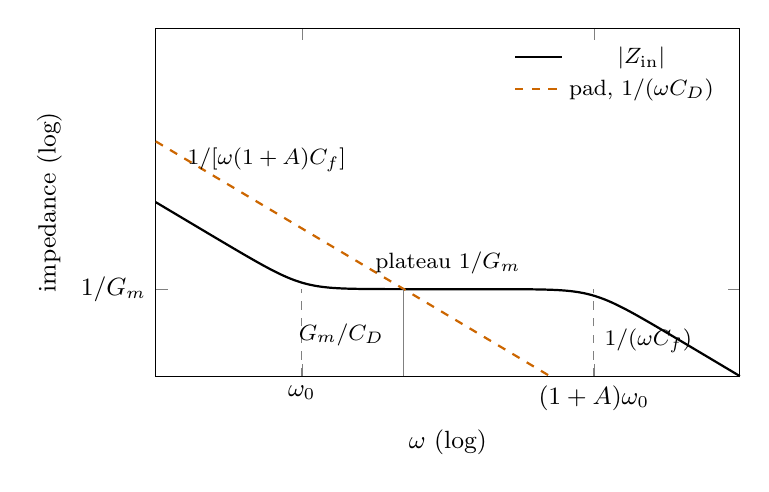
\begin{tikzpicture}[font=\small]
\begin{loglogaxis}[width=9cm,height=6cm,
  xmin=1e-2,xmax=1e6,ymin=1e-6,ymax=1e2,
  xtick={1,1e4},xticklabels={$\omega_0$,$(1+A)\omega_0$},
  ytick={1e-4},yticklabels={$1/G_m$},
  xlabel={$\omega$ (log)},ylabel={impedance (log)},clip=false,
  legend style={at={(0.98,0.98)},anchor=north east,draw=none,fill=none,font=\footnotesize},
  samples=300,domain=1e-2:1e6]
% normalised: Cf=1, w0=1, A=1e4, Gm=A*w0*Cf=1e4, CD=400 Cf
\addplot[black,thick] {sqrt(1+x^2)/(x*sqrt((1+1e4)^2+x^2))};
\addlegendentry{$|Z_{\rm in}|$}
\addplot[orange!80!black,thick,dashed,domain=1e-2:2.5e3] {1/(400*x)};
\addlegendentry{pad, $1/(\omega C_D)$}
\draw[dashed,gray] (axis cs:1,1e-6) -- (axis cs:1,1e-4);
\draw[dashed,gray] (axis cs:1e4,1e-6) -- (axis cs:1e4,1e-4);
\node[font=\footnotesize,anchor=south west] at (axis cs:2e-2,3e-2) {$1/[\omega(1+A)C_f]$};
\node[font=\footnotesize,anchor=north east] at (axis cs:3e5,2e-5) {$1/(\omega C_f)$};
\node[font=\footnotesize,anchor=south] at (axis cs:1e2,1.3e-4) {plateau $1/G_m$};
\draw[gray] (axis cs:25,1e-6) -- (axis cs:25,1e-4);
\node[font=\footnotesize,anchor=south east] at (axis cs:18,3e-6) {$G_m/C_D$};
\end{loglogaxis}
\end{tikzpicture}
\end{document}
